\section{Theoretical interpretation \label{sec:model}}

The search presented in this Letter is interpreted in terms of two benchmark simplified models: a Type-2 Two Higgs Doublet Model (2HDM)~\cite{Lee:1973iz,Branco:2011iw} where a vector \cPZpr\ is produced resonantly and decays into a Higgs boson plus an intermediate heavy pseudoscalar particle \Az, which decays into two DM particles; and a baryonic $\cPZpr_{B}$ model where a vector mediator $\cPZpr_{B}$ is exchanged in the s-channel, radiates a Higgs boson, and decays into two DM particles.

The Type-2 2HDM model is used to formulate
the Higgs sector. The gauge symmetry of the SM is extended by a
$U(1)_{\cPZpr}$ group, with a new massive \cPZpr\ gauge boson.
After electroweak symmetry breaking, the Higgs doublets attain vacuum
expectation values $v_u$ and $v_d$,
resulting in five physical Higgs bosons:
a light neutral CP-even scalar \Ph, assumed to be the
observed 125\GeV Higgs boson, a heavy neutral CP-even scalar \PH,
a neutral CP-odd scalar \Az, and two charged scalars \Hpm.

Only the masses \maz and \mzp affect the kinematic
properties of the physics objects studied in this search.

Mass hypotheses for the \cPZpr\ resonance are considered between 600 and 2500\GeV, and between 300 and 800\GeV for the \Az particle. The mass of the DM particles $m_{\chi}$
is assumed to be less than or equal to 100\GeV. The the
ratio of the vacuum expectation values of the two Higgs fields coupling to the up-type and down-type
quarks $\tan \beta$ and the coupling of the \Az particle to DM particles $g_{\chi}$ are fixed at unity. 
Hypotheses for the mass of the \Az particle to be less than 300\GeV are excluded by constraints on flavor changing
neutral currents from measurements of $\cPqb\rightarrow \cPqs\gamma$ \cite{Branco:2011iw},
and therefore are not considered. 
%The branching fraction of the \Az particle to dark matter, ${\cal B}(\Az\rightarrow\chi\overline{\chi})$, decreases as $m_{\chi}$ increases.
%For the mass range of the \Az particle considered in this paper, the relative drop of
%${\cal B}(\Az\rightarrow\chi\overline{\chi})$ when $m_{\chi}$
%increases from 0 to 100\GeV is within 7\% . Therefore, the result obtained with the assumption of $m_{\chi}= 100\GeV$ is considered valid also for $m_{\chi}\leq 100\GeV$.
%The value of ${\cal B}(\Az\rightarrow\chi\overline{\chi})$ is approximately $100\%$ for \Az particles of $300\GeV$ in mass.
%The branching fraction starts to decrease when the mass of the \Az particle is more than twice the mass
%of top quark, since the $\Az\rightarrow$ $\cPqt\cPaqt$ decay channel becomes kinematically
%accessible. For \Az particles of masses between if 400 and $800\GeV$ the branching fraction is reduced to values that range from 54 to $42\%$. In this paper 
The branching fraction ${\cal B}(\Az\rightarrow\chi\overline{\chi})$ is forced to be $100\%$ for all the considered mass hypotheses.
% and the results are presented in terms of exclusion limits of decays to
%DM particles and the signal cross section includes
%the value of ${\cal B}(\Az\rightarrow\chi\overline{\chi})$.
The signal cross sections are calculated for the fixed value of Z' gauge coupling $\gzp = 0.8$.
%, as considered in Ref.~\cite{ATLAS-2015-PAS} and recommended in
%Ref.~\cite{Abercrombie:2015wmb}. 

The baryonic $\cPZpr_{B}$ model is an extension of the SM and 
assumes that the baryon number B is gauged, with the Z' being the gauge 
boson of U(1)$_{B}$. The consistency of theory requires the existence of a new 
stable baryonic state that is neutral under SM gauge symmetry. This new 
particle is an excellent DM candidate. 
%If the DM particle carries a baryon 
%number $B_{\chi}$, the Z'-quark-DM part of the Lagrangian for models with 
%fermionic dark matter is 
%\begin{equation}
%{\cal L} = g_q \bar{q}\gamma^{\mu}q\cPZpr_{\mu}+g_{\chi}\bar{\chi}\gamma^{\mu}\chi\cPZpr_{\mu}
%\end{equation}
To generate the Z' mass, a ``baryonic Higgs'' scalar is introduced to 
spontaneously break the U(1)$_B$ symmetry. Analogous to the SM, there remains 
a physical baryonic Higgs particle, $h_{B}$, with a coupling of h$_{B}$Z'Z' 
and vacuum expectation value of v$_{B}$. 
The \cPZpr\ and SM Higgs boson h interact with a coupling strength of 
$g_{h\cPZpr\cPZpr} = m_{\cPZpr}^{2} \sin \theta/v_{B}$, where $\theta$ is the h-h$_{B}$ 
mixing angle. 
%This allows for mono-Higgs final states at the LHC as shown in 
%Fig.~\ref{fig:feynman}. 
In the search for this model, values for $g_q$ and $g_\chi$ are chosen to be 0.33 and 1, respectively. The ratio $g_{h\cPZpr\cPZpr}/M_{\mathrm{Z}'}$ is chosen to be unity. 
%All these parameter choices follow the recommendations from~\cite{Abercrombie:2015wmb}.  



%The quantity \ptvecmiss, calculated as the negative vectorial sum of the transverse momentum (\pt) of all objects identified in an event, 
%represents the total
%momentum carried by the DM particles.
%The magnitude of this vector is referred to as \MET.
%For a given value of \mzp, the \pt of the \Az decreases as its mass increases.
%Therefore, the \MET spectrum softens with increasing \Az masses.
%A comparison of the \MET distributions expected from representative scenarios of the \cPZpr-2HDM model and the \cPZpr-Barzonic model are presented in Fig.~\ref{fig:met_signals}.


%\begin{figure}
%\centering
%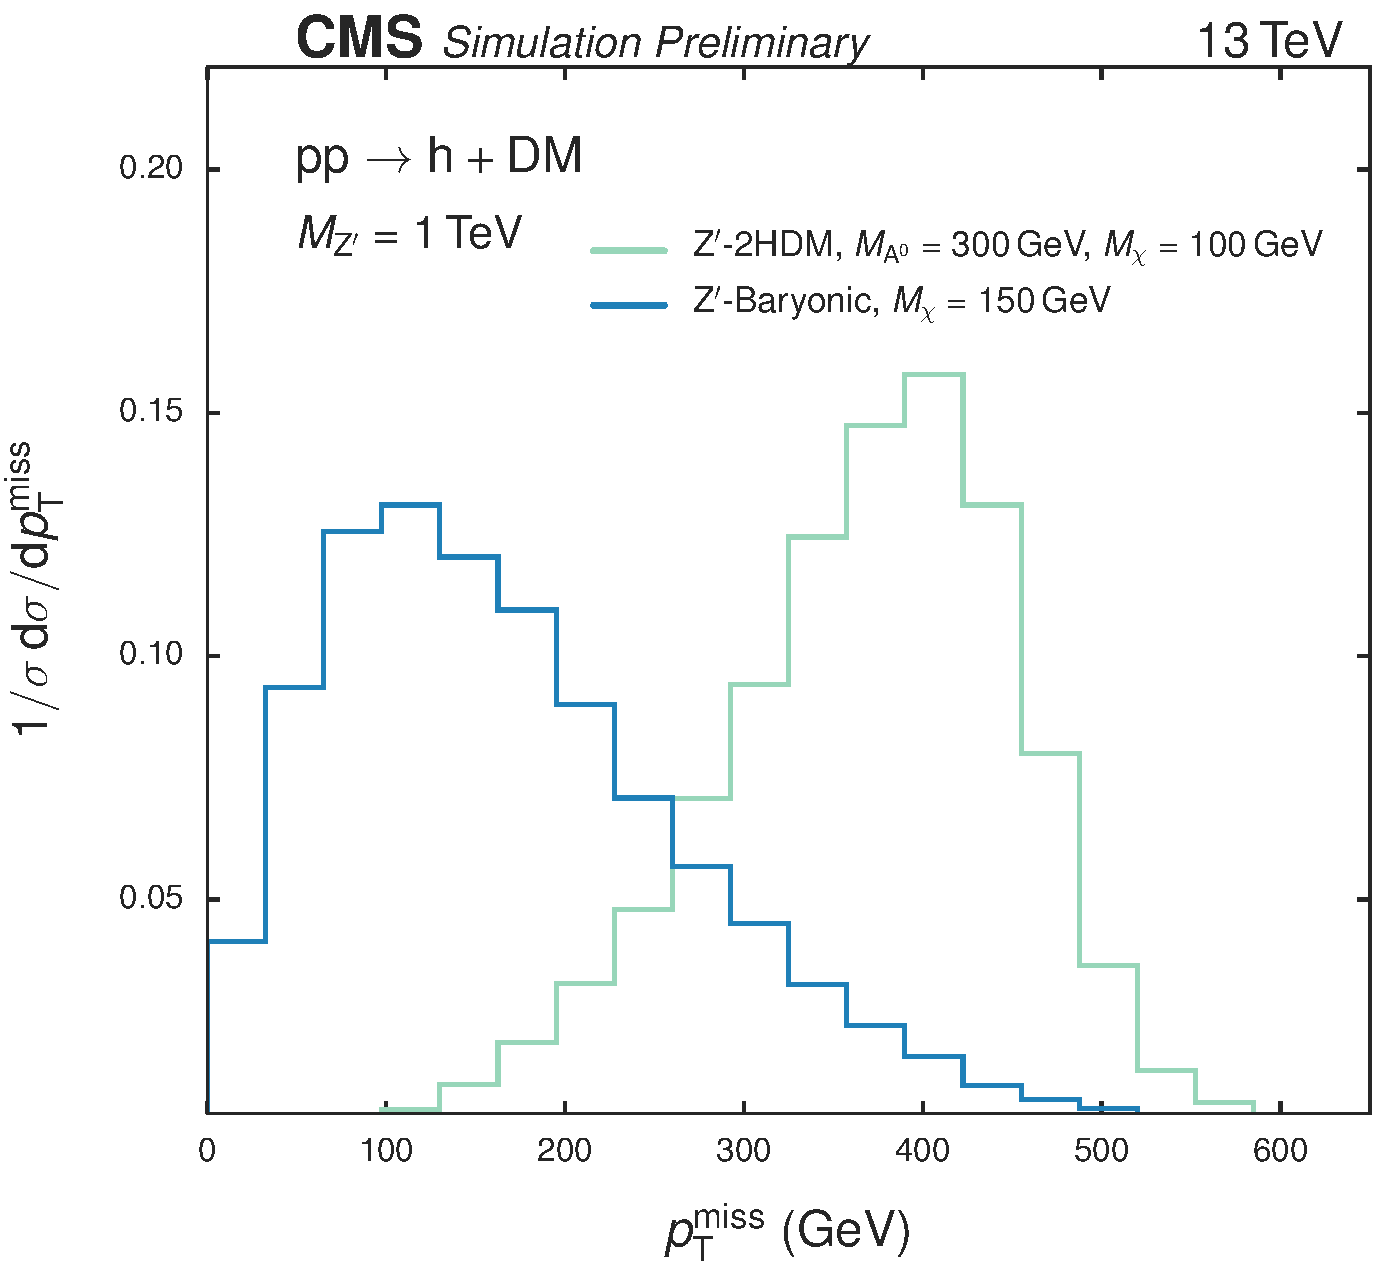
\includegraphics[width=0.55\textwidth]{figures/puppimet_signals.pdf}
%\includegraphics[width=0.45\textwidth]{figures/ZpBaryonicModel.pdf}
%\caption{Reconstructed \MET for representative scenarios of two $\mathrm{h}+\mathrm{DM}$ models investigated. Coupling parameters are chosen as mentioned in the text. The \cPZpr-2HDM model in general has a significant harder \MET~spectrum than the \cPZpr-Barzonic model, which makes the former easier to distinguish from SM background processes.}
%\label{fig:met_signals}
%\end{figure}

